\documentclass[runningheads,a4paper]{llncs}

\usepackage{latexsym}
\usepackage{setspace}
\usepackage{cancel}
\usepackage{listings}
\usepackage{graphicx}
\usepackage{appendix}
\usepackage{amssymb}
\usepackage{stmaryrd}
\usepackage{amsmath}
\usepackage{leftidx}
\usepackage{mathtools}
\usepackage[linesnumbered,noend]{algorithm2e}
\usepackage{paralist}
\usepackage{color}
\usepackage{mathrsfs}
\usepackage{tikz}
\usetikzlibrary{shapes}
%\usepackage{times}
\newcommand{\hide}[1]{}

\newcommand{\eval}[2]{\llbracket#1\rrbracket_{#2}}
\newcommand\cur{\mathsf{cur}}
\newcommand\dom{\mathsf{dom}}
\newcommand\rng{\mathsf{rng}}

\newcommand\dd{\mathbb{D}}
\newcommand\nat{\mathbb{N}}

\newcommand\Ss{\mathcal{S}}


\newcommand\vard{\mathfrak{d}}



\newcommand{\yfc}[1]{\color{blue} {YF: #1 :FY} \color{black}}
\newcommand{\zhilin}[1]{\color{cyan} {ZL: #1 :LZ} \color{black}}
\newcommand{\tl}[1]{\color{green} {TL: #1 :LT} \color{black}}

\title{Streaming data transducers}
\titlerunning{}
\author{}
\institute{}

\author{Taolue Chen, Yu-Fang Chen, Anthony Widjaja Lin, Zhilin Wu}
\begin{document}

\maketitle


\begin{abstract}
In this note, as a starting point, we define a model called streaming data transducers (SDT), which on the one hand ignores the guards in the corresponding model introduced in the cav paper, and on the other hand extends the model by introducing data grammars and data models. The SDT model can be seen as an extension of cost register automata (Rajeev Alur, Loris D'Antoni, Jyotirmoy Deshmukh, Mukund Raghothaman,  and Yifei Yuan, LICS 2013) to data words. The model presented here is tentative and presented just as a material for discussions and a catalyst for more interesting results in the near future.
\end{abstract}



\section{Data grammar and data model}

%\begin{remark}
{\bf Warning}: Most of the notations are adapted from those of cost register automata \cite{ADD+13}.
%\end{remark}

For each $n \in \nat$, let $[n]=\{1,\dots, n\}$.

An infinite data domain $\dd$ is fixed.
A ranked alphabet $F$ is a finite set of function symbols, each of which has a fixed arity. The arity-0 symbols are called constants, are mapped to the elements in the data domain. Since infinite data domains are allowed, we need a way of encoding the constants as strings as a finite set of symbols (e.g. the set of symbols is $\{0,1\}$, and $3$ is encoded as $11$), but we will not go into details here. In addition, we assume a  finite set of variables $X$ ranging over $\dd$.  The set of terms over $F$ and $X$, denoted by $T_{F, X}$, can defined in a standard way, more specifically, by the grammar $t::= c \mid x  \mid f(t_1,\dots, t_k)$, where $c$ is a constant symbol in $F$, $x \in X$, and $f \in F$ is a function symbol in $F$ of arity $k$. A \emph{data grammar} $G$ is a pair $(F, T)$, where $F$ is a ranked alphabet, $T \subseteq T_{F,X}$ such that $T$ is a regular tree language over the alphabet $F \cup X$, where each element of $X$ is taken as the arity-0 symbols.  A \emph{valuation} of $Z$ is a function $\rho$ from $Z$ to $\dd$. For a valuation $\rho$ of $X$, $x \in X$, and $d \in \dd$, we use $\rho[d/x]$ to denote the valuation which is the same as $\rho$, except assigning $d$ to $x$.

\begin{example}
Here are a few examples of data grammars.
\begin{itemize}
\item Additive grammar $G_+=(F, T)$, where $F=\{c_1,\dots, c_k, +\}$ and $T=T_{F,X}$. 

\item Increment grammar $G_{\sf inc} = (F, T)$, where $F=\{c_1,\dots, c_k, +\}$, and $T$ is defined by the rules $t ::= c_i \mid x \mid +(t, c_i)$ (here $c_i \in F$ and $x \in X$). 

\item Max-increment grammar $G_{\sf max-inc} = (F, T)$, where $F=\{c_1,\dots, c_k, \max, +\}$, and $T$ is defined by the rules $t ::= c_i \mid x \mid \max(t_1, t_2) \mid +(t,c_i)$ (here $c_i \in F$ and $x \in X$). 

\item Data grammar $G_\otimes = (F,T)$, where $F=\{0, \otimes\}$ (here $0$ is a constant and $\otimes$ is an arity-2 symbol), and $T=T_{F,X}$. 
\end{itemize}
\end{example}

Given a data grammar $G=(F, T)$, a \emph{data model} is a triple $(G, \dd, \llbracket \cdot \rrbracket)$, where $\dd$ is a data domain,  for each constant $c \in F$, $\llbracket c\rrbracket \in \dd$, and for each arity-$k$ ($k > 0$) function symbol $f \in F$, $\llbracket f \rrbracket $ is a function from $\dd^k$ to $\dd$. 

\begin{example}
$(G_+, \nat, \llbracket \cdot \rrbracket)$ denotes the data model where $\dd=\nat$ and $\llbracket + \rrbracket$ is interpreted as the standard addition operation. Monoid data model $(G_\otimes, \dd, \llbracket \cdot \rrbracket)$ where $(\dd, 0, \llbracket \otimes \rrbracket)$ is a monoid (this means that $ \llbracket \otimes \rrbracket$ is an associative operation on $\dd$). In particular, the monoid $(\dd, 0, \llbracket \otimes \rrbracket)$ in the monoid data model can be instantiated as $(\Sigma^\ast, \varepsilon, \cdot)$, where $\cdot$ denotes the string concatenation operation. Commutative-monoid data model $(G_\otimes, \dd, \llbracket \cdot \rrbracket)$ where $(\dd, 0, \llbracket \otimes \rrbracket)$ is a commutative monoid (this means that $\llbracket \otimes \rrbracket$ is an associative and commutative operation). The commutative-monoid  $(\dd, 0, \llbracket \otimes \rrbracket)$ can be instantiated as $(\nat, 0, +)$, and $(\nat, 1, \times)$. 
\end{example}

Suppose $t \in T$, and $\rho$ is a valuation of $Z$. Then $t$ naturally defines a data value in $\dd$ w.r.t. $\llbracket \cdot \rrbracket$ and $\rho$ (this data value is denoted by $\eval{t}{\rho}$). For instance, in the data model $(G_+, \nat, \llbracket \cdot \rrbracket)$ where $\llbracket + \rrbracket$ is the addition operation on $\nat$, if $\rho(x) = 5$, then $\eval{+(2,x)}{\rho}=7$.

 
\section{Streaming data transducer (SDT)}

We assume that $X$ contains a special variable $\cur$ to denote the data value in the current position. 

%We use $X^+$ to denote $X \cup \{\cur\}$.

A streaming data transducer (SDT) over a data model $(G=(F, T), \dd, \llbracket \cdot \rrbracket)$ is a tuple $(Q, X, \delta, q_0, O)$, where 
\begin{itemize}
\item $Q$ is a finite set of states, 

\item $X$ is a finite set of variables such that $\cur \in X$, 

\item $\delta$ is a partial function which maps a state $q \in Q$ to a tuple $(q',\eta)$  such that $q' \in Q$ and $\eta$ is an assignment function which assigns to each $x \in X$ a term $\eta(x) \in T$, 

\item $q_0 \in Q$ is the initial state, 

\item $O$ is the output function which is a partial function such that for each $q \in \dom(O)$, $O(q) \in T$ is a term denoting the output where the variable $\cur$ does not occur.
\end{itemize}
Note that since an SDT $\Ss$ defined above is required to be deterministic and the guards are disallowed at present, the shape of the transition graph of $\Ss$ is either a simple path or a lasso. For convenience, we write a transition $\delta(q) = (q',\eta)$ as $q \xrightarrow{\eta} q'$.


The semantics of an SDT $S = (Q, Z, \delta, q_0, O)$  is defined as follows. We assume that the data domain $\dd$ always contain a special constant $0$. A \emph{configuration} of $S$ is a pair $(q, \rho)$, where $q \in Q$ and $\rho$ is a valuation of $Z$. The \emph{initial} configuration of $S$ is $(q_0,\rho_0)$, where $\rho_0(z)=0$ for each $z \in X$. A sequence of configurations $(q_0,\rho_0)(q_1,\rho_1)\ldots(q_n,\rho_n)$ is
a \emph{run} of $S$ over a data word $w=d_1 \dots d_n$ iff there exists a path (sequence of transitions) $q_0 \xrightarrow{\eta_1} q_1 \xrightarrow{(g_2,\eta_2)} q_2 \dots q_{n-1} \xrightarrow{(g_n, \eta_n)} q_n$ such that for each $i \in [n]$, $\rho_i$ is obtained from $\rho_{i-1}[d_i/\cur]$ as follows: For each $z \in Z$, $\rho_i(z)=\eval{\eta_i(z)}{\rho_{i-1}[d_i/\cur]}$.
We call $(q_n,\rho_n)$ the \emph{final configuration} of the run. %We say that $(q_i,\rho_i)$ is \emph{reachable} from $(q_0,\rho_0)$, for $i \in [n]$.

%The semantics of an SDT $S = (Q, Z, \delta, q_0, O)$  is defined as follows. We assume that the data domain $\dd$ always contain a special constant $0$. A \emph{configuration} of $S$ is a pair $(q, \rho)$, where $q \in Q$ and $\rho$ is a valuation of $Z$. The \emph{initial} configuration of $S$ is $(q_0,\rho_0)$, where $\rho_0(z)=0$ for each $z \in X$. A sequence of configurations $(q_0,\rho_0)(q_1,\rho_1)\ldots(q_n,\rho_n)$ is
%a \emph{run} of $S$ over a data word $w=d_1 \dots d_n$ iff there exists a path (sequence of transitions) $q_0 \xrightarrow{\eta_1} q_1 \xrightarrow{(g_2,\eta_2)} q_2 \dots q_{n-1} \xrightarrow{(g_n, \eta_n)} q_n$ such that for each $i \in [n]$, $\rho_{i-1}[d_i/\cur] \models g_i$, and $\rho_i$ is obtained from $\rho_{i-1}$ as follows: For each $x \in X$, if $x \in \dom(\eta_i)$, then $\rho_i(x)=\eval{\eta_i(x)}{\rho_{i-1}[d_i/\cur]}$, otherwise, $\rho_i(x)=\rho_{i-1}(x)$.
%We call $(q_n,\rho_n)$ the \emph{final configuration} of the run.

We would like to remark that for each data word $w$, there is at most one run of $S$ over $w$, since $S$ is deterministic. 
Over a data word $w = d_1 \dots d_n$, if there is a run of $S$ over $w$ with the final configuration $(q_n,\rho_n)$, and $O(q_n)$ is defined, then the output of $S$ over $w$, denoted by ${S}(w)$, is $\eval{O(q_n)}{\rho_n}$. Otherwise, ${S}(w)$ is $\bot$.

We focus on three decision problems of SDTs: (1) \emph{Commutativity}: Given an SDT $S$, decide whether $S$ is commutative, that is, whether for each data word $w$ and each permutation $w'$ of $w$, $S(w)=S(w')$. (2) \emph{Equivalence}: Given two SDTs $S_1,S_2$, decide whether $S_1$ and $S_2$ are equivalent, that is, whether over each data word $w$, $S_1(w)=S_2(w)$.


\begin{example}
If we assume the monoid data model $(G_\otimes, \dd, \llbracket \cdot \rrbracket)$ where $(\dd, 0, \llbracket \otimes \rrbracket)$  is interpreted as $(\Sigma^\ast, \varepsilon, \cdot)$, then we get streaming transducers in \cite{RP11} (without guards), whose output are data strings. If we assume the commutative data model $(G_\otimes, \dd, \otimes)$, then we get a model similar to streaming numerical transducers in the cav paper (without guards).
\end{example}

Since the commutativity problem of SDTs can be reduced the equivalence problem, we focus on the equivalence problem of SDTs in the following.

\section{Equivalence problem: A first dive}

We will try to get some idea on the equivalence problem by considering the special case that the data grammar $G=(F,T)$, where $F=\{f\}$, where $f$ is an arity-2 function symbol and $T = T_{F,X}$. We will consider free data model where $f$ is an arbitrary binary function on $\dd$, the commutative data model where $\llbracket f \rrbracket$ is a commutative binary operation on $\dd$, the monoid and commutative-monoid data model, that is, $(\dd, 0, \llbracket f \rrbracket)$ is a monoid resp. commutative monoid.

Suppose that $(G, \dd, \llbracket \cdot \rrbracket)$ is data model, $\Ss_1 = (Q_1, Z_1, \delta_1, q_{1,0}, O_1)$ and $\Ss_2 = (Q_2, Z_2, \delta_2, q_{2,0}, O_2)$ are two SDTs over $(G, \dd, \llbracket \cdot \rrbracket)$. Without loss of generality, we assume that for $i=1,2$, the transition graph of $\Ss_i$ is a lasso 
$$q_{i,0} \xrightarrow{\eta_{i,1}} q_{i, 1}  \dots q_{i, h_i} \xrightarrow{\eta_{i, h_i+1}} q_{i, h_i+1} \dots \xrightarrow{\eta_{i, h_i+p_i}} q_{i, h_i+p_i}$$ 
such that $q_{i, h_i+p_i}= q_{i, h_i}$. The path $q_{i,0} \xrightarrow{\eta_{i,1}} q_{i, 1}  \dots q_{i, h_i}$ is called the \emph{handle} and $q_{i, h_i} \xrightarrow{\eta_{i, h_i+1}} q_{i, h_i+1} \dots \xrightarrow{\eta_{i, h_i+p_i}} q_{i, h_i+p_i}$ is called the \emph{loop} of the lasso. In addition, $h_i$ and $p_i$ are called the length of the handle and loop respectively.

Let $h=\max(h_1,h_2)$ and $p = {\sf lcm}(p_1, p_2)$. Then we can transform $\Ss_1$ and $\Ss_2$ into $\Ss'_1$ and $\Ss'_2$ such that the transition graphs of $\Ss'_1$ and $\Ss'_2$ are of the same shape, that is, the two handles of $\Ss'_1$ and $\Ss'_2$ have the same length $h$ and the two loops of the lassos in $\Ss'_1$ and $\Ss'_2$ both have length $p$.

\begin{example}
Suppose the transition graph of $\Ss_1$ is $q_{1,0} \xrightarrow{\eta_{1,1}} q_{1, 1}  \xrightarrow{\eta_{1,2}} q_{1, 2} \xrightarrow{\eta_{1, 3}} q_{1, 3} \xrightarrow{\eta_{1, 4}} q_{1, 2}$, and the transition graph of $\Ss_2$ is 
$q_{2,0} \xrightarrow{\eta_{1,1}} q_{2, 1}  \xrightarrow{\eta_{2,2}} q_{2, 2} \xrightarrow{\eta_{2, 3}} q_{2, 3} \xrightarrow{\eta_{2, 4}} q_{2, 1}$. Then $\Ss_1$ can be transformed into $\Ss'_1$ with the transition graph $q_{1,0} \xrightarrow{\eta_{1,1}} q_{1, 1}  \xrightarrow{\eta_{1,2}} q_{1, 2} \xrightarrow{\eta_{1, 3}} q_{1, 3} \xrightarrow{\eta_{1, 4}} q'_{1, 2} \xrightarrow{\eta_{1, 3}} q'_{1, 3} \xrightarrow{\eta_{1, 4}} q''_{1, 2}  \xrightarrow{\eta_{1, 3}} q''_{1, 3} \xrightarrow{\eta_{1, 4}} q_{1, 2}$, where $q'_{1,2}, q'_{1, 3}, q''_{1, 2}, q''_{1, 3}$ are freshly introduced states. In addition, $\Ss_2$ is transformed into $\Ss'_2$ with the transition graph $q_{2,0} \xrightarrow{\eta_{2,1}} q_{2, 1}  \xrightarrow{\eta_{2,2}} q_{2, 2} \xrightarrow{\eta_{2, 3}} q_{2, 3} \xrightarrow{\eta_{2, 4}} q'_{2, 1} \xrightarrow{\eta_{2, 2}} q'_{2, 2} \xrightarrow{\eta_{2, 3}} q'_{2, 3}  \xrightarrow{\eta_{2, 4}} q''_{2, 1} \xrightarrow{\eta_{2, 2}} q_{2, 2}$, where $q'_{2,1}, q'_{2,2}, q'_{2,3}, q''_{2,1}$ are the freshly introduced states. Note that the output functions $O_1$  and $O_2$ should be adjusted accordingly.
\end{example}

Therefore, in the rest of this section, we assume that the two transition graphs of $\Ss_1$ and $\Ss_2$ have the same shape, that is, $h_1 = h_2 = h$ and $p_1 = p_2 = p$. Moreover, we use $H_1, L_1$ and $H_2,L_2$ to denote the handle and loop of $\Ss_1$ and $\Ss_2$ respectively.

Without loss of generality, we assume that $Z_1 \cap Z_2 = \emptyset$, $Z_1 = \{z_1, \dots, z_{k_1}\}$ and $Z_2 = \{z'_1,\dots, z'_{k_2}\}$. Let $\Ss$ be the product of $\Ss_1$ and $\Ss_2$, ignoring the output function, that is, $\Ss=(Q= Q_1 \times Q_2, Z= Z_1 \cup Z_2, \delta, (q_{1,0}, q_{2,0}))$ where for each $(q_1,q_2) \in Q_1 \times Q_2$, if $\delta(q_1)=(q'_1,\eta_1)$ and $\delta(q_2)=(q'_2, \eta_2)$, then $\delta(q_1, q_2)=((q'_1,q'_2), \eta_1 \cup \eta_2)$. Note that since the transition graphs of $\Ss_1$ and $\Ss_2$ have the same shape, we know that the transition graph of $\Ss$ is also a lasso whose handle and loop are of the length $h$ and $p$ respectively. We use $H$ and $L$ to denote the handle and loop of $\Ss$.

We illustrate the argument by considering the special case that $O_1(q_{1,h})=z_1$, $O_2(q_{2,h})=z'_1$, and $O_1(q'_1)$ and $O_2(q'_2)$ are undefined  for all the other states $q'_1  \in Q_1$ and $q'_2 \in Q_2$.

 
\subsection{Free data model}

\hide{
For $i=1,2$, define 
$$I_{\Ss_i} = \{j \mid 1 \le j \le h, q_{i,j} \in \dom(O) \} \cup \{h + n p + j \mid n \in \nat, 0 \le j < p, q_{i, h+j} \in \dom(O)\}.$$

\smallskip

\noindent {\bf Step I}: If $I_{\Ss_1} \neq I_{\Ss_2}$, then return false. Otherwise, go to Step II.

\smallskip
}


We will show that if there is data word $w$ such that $\Ss_1(w) \neq \Ss_2(w)$, then there is a data word $w'$ of bounded length such that $\Ss_1(w') \neq \Ss_2(w')$.

The effect of the handle $H$ on each $z \in Z$ can be summarized by an expression $\eta_H(z)$ which is a term where the variables from $Z_1 \cup Z_2 \cup \{\vard_1,\dots, \vard_h\}$ occur, where $\vard_1,\dots, \vard_h$ are $h$ fresh variables introduced to represent the $h$ data values met when traversing the handle.  Let $D_H = \max_{z \in Z} {\sf depth}(\eta_H(z))$, where ${\sf depth}(\eta_H(z))$ denote the  maximum length of paths in the term $\eta_H(z)$.

At first, we observe the following fact.

\begin{proposition}\label{prop-distinct}
If there is data word $w$ such that $\Ss_1(w) \neq \Ss_2(w)$, then there is a data word $w'$ such that  no two positions of $w'$ hold the same data value and $\Ss_1(w') \neq \Ss_2(w')$.
\end{proposition}

\newcommand\node{{\sf Node}}

\newcommand\dif{{\sf DIF}}

\newcommand\var{{\sf var}}

We then show the small path property for the equivalence problem.

\begin{proposition}\label{prop-free-bnd}
If there is data word $w$ such that $\Ss_1(w) \neq \Ss_2(w)$, then there is a data word $w'$ of length no greater than $h+(2D_H |Z_1|  |Z_2|)p$  such that $\Ss_1(w') \neq \Ss_2(w')$.
\end{proposition}

\begin{proof}
Suppose that $w = d_1 \dots d_n$ is data word such that $n > h+(2D_H |Z_1|  |Z_2|)p$, no two positions of $w$ hold the same data value, and $\Ss_1(w) \neq \Ss_2(w)$. Without loss of generality, we assume that none of the data values occurring in $w$ is equal to a constant occurring in $\Ss_1$ or $\Ss_2$.  Note that $\Ss_1(w)$ and $\Ss_2(w)$ are terms labeled by the constants, the function symbol $f$, and the data values $d_1,\dots,d_n$. For each path $\pi \in \{l, r\}^+$ (where $l,r$ denote the left and right branch respectively), let $\Ss_1(w)[\pi]$ denote the label of the node of $\Ss_1(w)$ corresponding to $\pi$. Similarly for $\Ss_2(w)[\pi]$. Since $\Ss_1(w) \neq \Ss_2(w)$, there are two maximal paths $\pi_1,\pi_2 \in \{l, r\}^+$ in $\Ss_1(w)$ and $\Ss_2(w)$ respectively such that $\pi_1$ is a prefix of $\pi_2$ and $\Ss_1(w)[\pi_1] \neq \Ss_2(w)[\pi_1]$, or $\pi_2$ is a prefix of $\pi_1$ and $\Ss_1(w)[\pi_2] \neq \Ss_2(w)[\pi_2]$. Without loss of generality, we assume that $\pi_1$ is a prefix of $\pi_2$ and $\Ss_1(w)[\pi_1] \neq \Ss_2(w)[\pi_1]$. 
This implies that one of $\Ss_1(w)[\pi_1]$ has to be some constant $c$ or some data value $d_i$.


Suppose on $w$, the loop of $\Ss_1$ (resp. $\Ss_2$) is iterated for $N \in \nat$ times.  Then the path $\pi_1$ can be divided into segments $\pi_{1,0}, \pi_{1,1}, \dots, \pi_{1,N}$, where $\pi_{1,N}$ is the path corresponding to the handle $H$, $\pi_{1,N-1}, \dots, \pi_{1,0}$ correspond to the first, second, and $N$-th iteration of the loop. Similarly $\pi_2$ can be divided into $\pi_{2,0}, \pi_{2,1}, \dots, \pi_{2,N}$. Moreover, the data word $w$ can also be divided into $w_0 w_1 \dots w_N$ such that $|w_0| = h$ and $|w_1|=\dots = |w_N|=p$.

For each $1 \le j < N$, define $\dif_{j}$ as $ (\sum \limits_{0 \le j' \le j} |\pi_{1,j'}|) - (\sum \limits_{0 \le j' \le j} |\pi_{2,j'}|) $. 

If $|\dif_j| > D_H$ ($|\dif_j|$ is the absolute value of $\dif_j$) for some $j < N$, then return false ($\Ss_1$ and $\Ss_2$ are not equivalent). The reason is that in this case, let $z_1 \in Z$  and $z_2 \in Z$ be the variable in the node $\pi_{1,0} \dots \pi_{1,j}$ of $\Ss_1(w)$ and  $\pi_{2,0} \dots \pi_{2,j}$ of $\Ss_2(w)$ respectively, that is, the value of the variable $z_1$ and $z_2$ are used in the $(N-j)$-th iteration of the loop in $\Ss_1$ and $\Ss_2$ respectively. Then we can replace the subterm rooted at $\pi_{1,0} \dots \pi_{1,j}$ by $\eta_H(z_1)$ in $\Ss_1(w)$, and the subterm rooted at $\pi_{2,0} \dots \pi_{2,j}$ by $\eta_H(z_2)$ in $\Ss_2(w)$, then the resulting two terms are still different, even we do some replacements in other places of the two trees, but without modifying the paths $\pi_{1,0} \dots \pi_{1, j}$  and $\pi_{2,0} \dots \pi_{2, j}$.  Let  $w' = w_0 w_{N-j} \dots w_N$. Then $\Ss_1(w') \neq \Ss_2(w')$, that is, we get a shorter data word witnessing the non-equivalence of $\Ss_1$ and $\Ss_2$.

Otherwise, for each $j < N$,  $\dif_j \le D_H$. For each $j < N$, let $\var_{1,j} \in Z_1$ (resp. $\var_{2,j} \in Z_2$) denote the variable of $\Ss_1$ (resp. $\Ss_2$) corresponding to the path $\pi_{1,0} \dots \pi_{1,j}$ (resp. $\pi_{2,0} \dots \pi_{2,j}$) respectively. Let us consider the tuples $(\var_{1,j}, \var_{2,j}, \dif_j)$ for $j < N$. Then these tuples belong to $Z_1 \times Z_2 \times [-D_H, D_H]$. Since $n  > h+(2D_H |Z_1|  |Z_2|)p$,  we know that $N > 2D_H |Z_1|  |Z_2|$. 
Then there must be $0 \le j_1 < j_2 < N$ such that $(\var_{1, j_1}, \var_{2, j_1}, \dif_{j_1}) = (\var_{1, j_2}, \var_{2, j_2}, \dif_{j_2})$. We can shrink the segment $\pi_{1, j_1+1} \dots \pi_{1,j_2}$ from $\Ss_1(w)$ and   $\pi_{2, j_1+1} \dots \pi_{2,j_2}$ from $\Ss_2(w)$ respectively, so that the resulting pair of terms are still different. Let $w' = w_0 w_1 \dots w_{N-j_2-1} w_{N- j_1} \dots w_N$. Then we get a data word $w'$ of shorter length witnessing the non-equivalence of $\Ss_1$ and $\Ss_2$. 
\qed
\end{proof}


\subsection{Commutative data model}


\subsection{Reduction to two-player reachability games: free data model and commutative data model}

Let us use the following example to illustrate the idea.

Let $\Ss_1$ and $\Ss_2$ be two SDTs such that they are self-loops around $q_1$ and $q_2$ with the transitions 
$\left(\begin{array}{l c l} x_1 &=& f(x_3, x_2) \\ x_2 &=& f(1, x_1) \\ x_3 &=& f(2, x_1) \end{array}\right)$
and
$\left(\begin{array}{l c l} y_1 &=& f(y_2, y_3) \\ y_2 &=& f(1,y_1) \\ y_3 &=& f(2, y_1)\end{array}\right)$
respectively. In addition, let $O(q_1)=x_1$ and $O(q_2)=y_1$. We assume that the initial values of all the variables are the constant $0$. Then the equivalence of $\Ss_1$ and $\Ss_2$ is reduced to a two-player reachability game $(V_1, V_2, E)$ illustrated in Fig.~\ref{fig-equiv-to-game}, where the goal of Player 1 is to defend the fact that for each data word $w$, the run of $\Ss_1$ and $\Ss_2$ on $w$ produce the same output (that is, $x_1$ and $y_1$ have the same value) and the goal of Player 2 is to attack this fact. It is easy to see that Player 2 has a winning strategy starting from $(x_1, y_1)$.
\begin{figure}[h]
\begin{center}
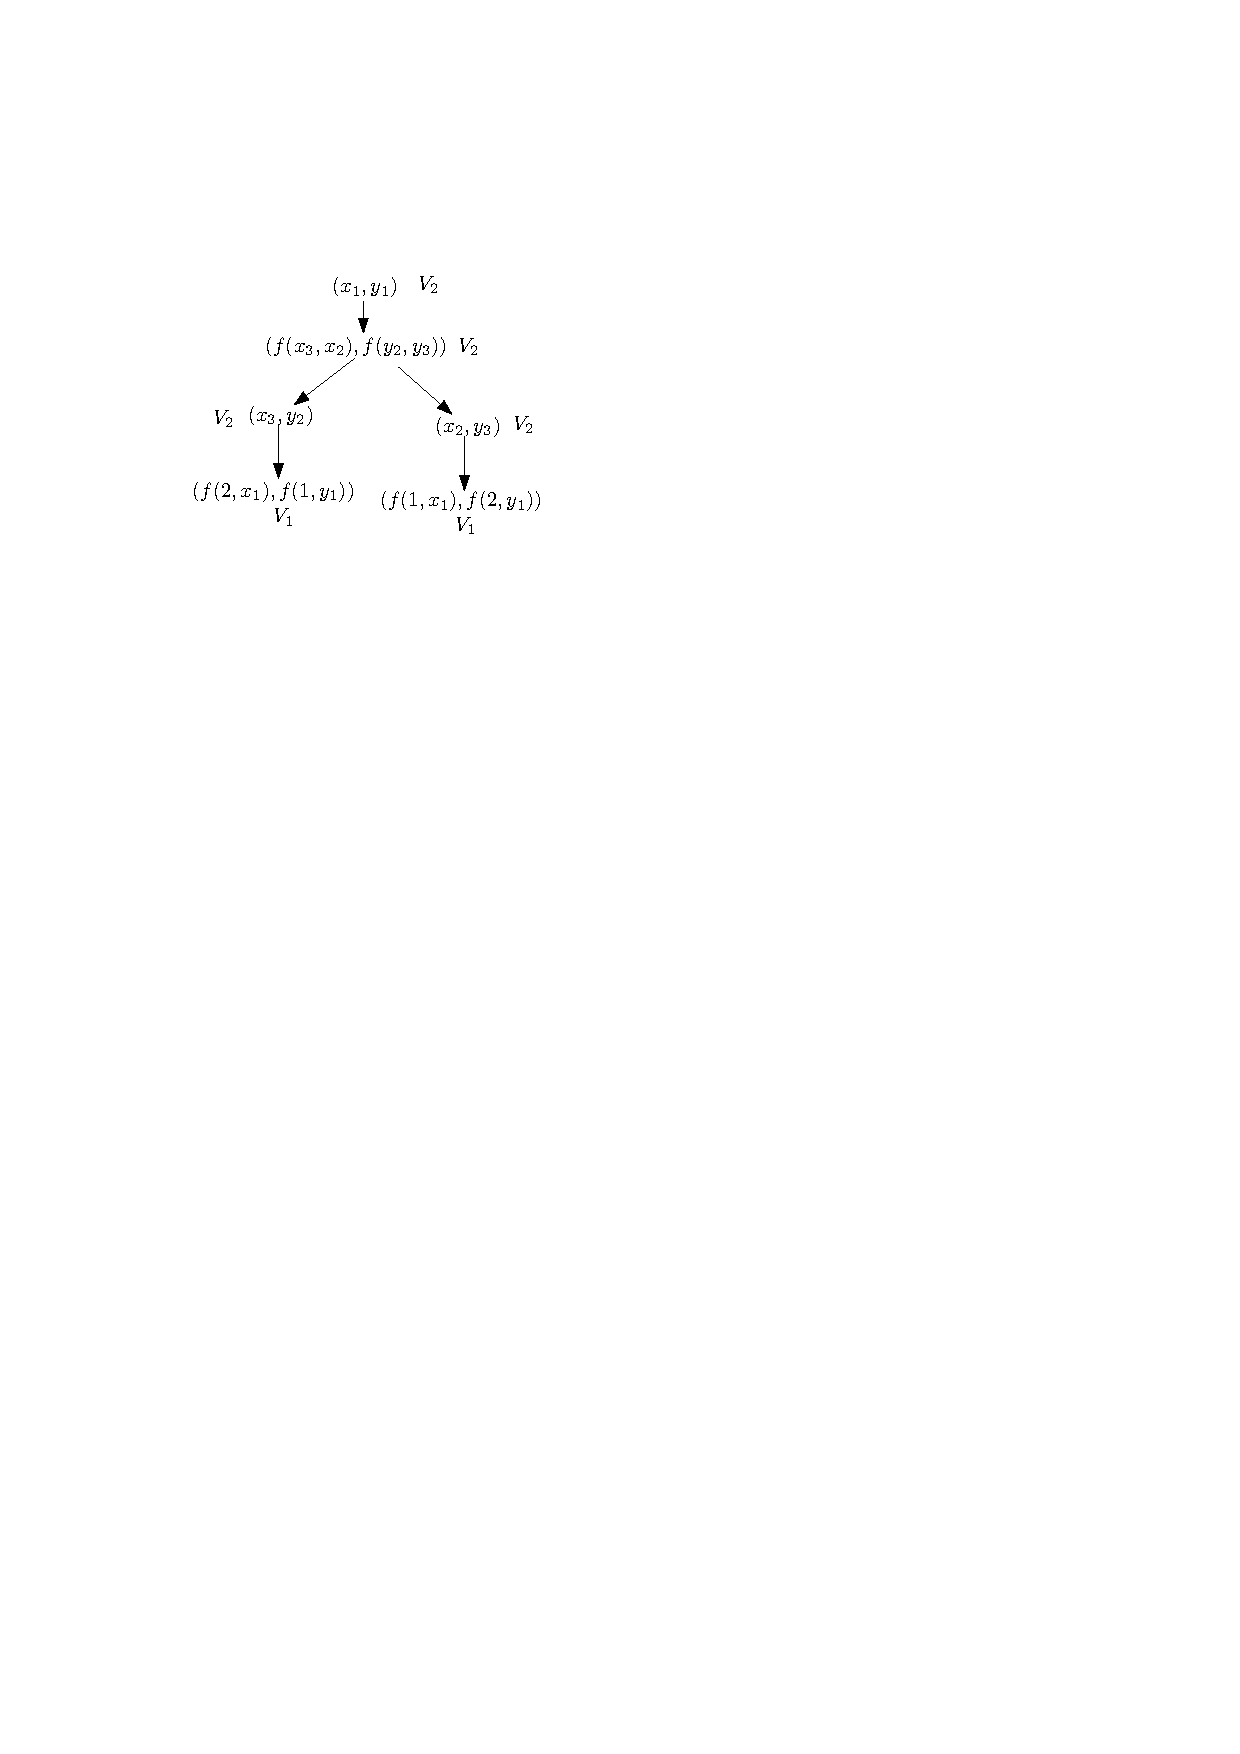
\includegraphics[scale=0.9]{game.pdf}
\end{center}
\caption{From equivalence to two-player reachability game: Free data model}\label{fig-equiv-to-game}
\end{figure}

If we assume that $f$ is commutative, then we can reduce the equivalence of $\Ss_1$ and $\Ss_2$ to another two-player reachability game illustrated in Fig.~\ref{fig-equiv-to-game-com}. It is easy to see that Player 1 has a winning strategy starting from $(x_1, y_1)$.
\begin{figure}[h]
\begin{center}
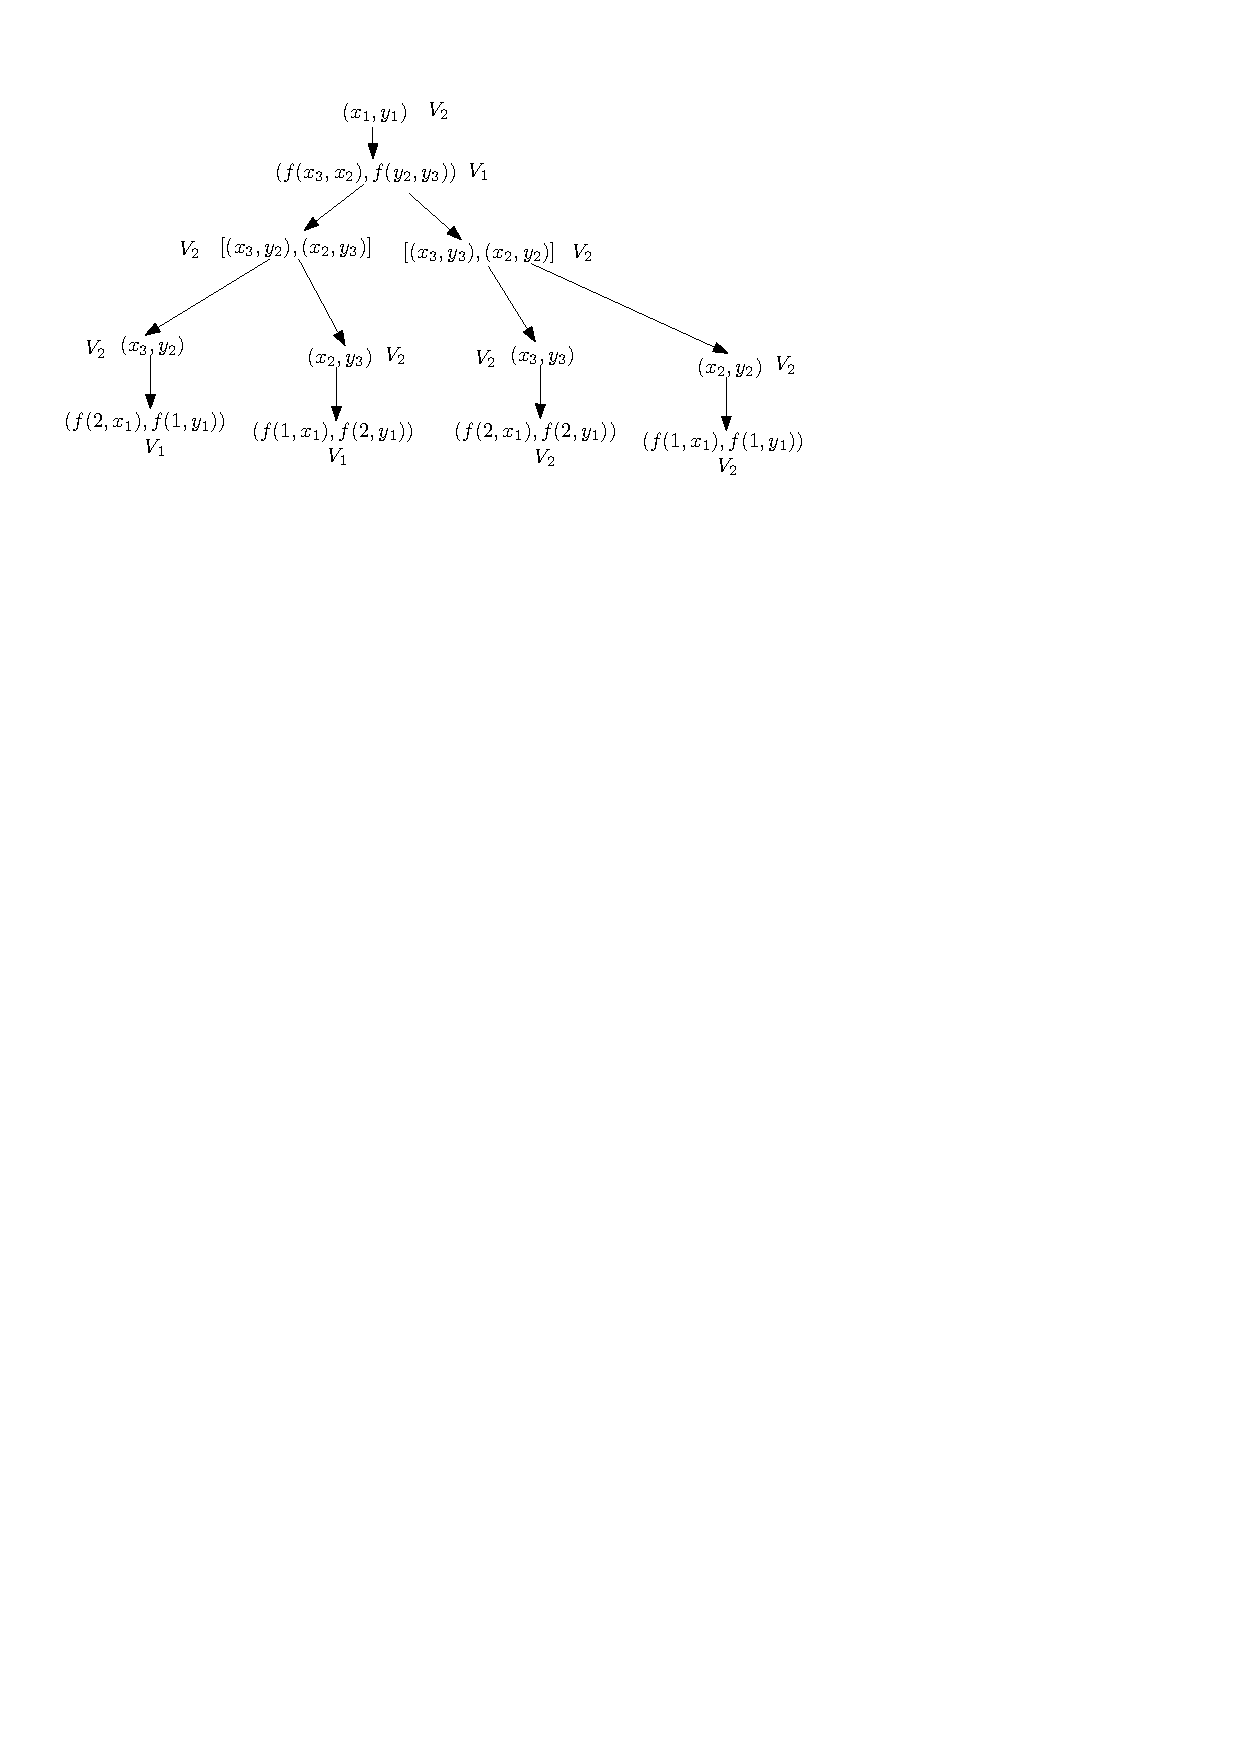
\includegraphics[scale=0.9]{game-com.pdf}
\end{center}
\caption{From equivalence to two-player reachability game: Commutative data model}\label{fig-equiv-to-game-com}
\end{figure}


\subsection{Monoid data model}

Essentially decide the frontiers of two trees are equal.

\subsection{Commutative-monoid data model}

Essentially decide the Parikh images of the frontiers of two trees are equal. 

\hide{
\section{Follow-up discussion}

If recall correctly, we have discussed the simple case that there is a simple loop for SNT. The aim is to generate a ``satisfactory representation" of the output function. At a very high level, we have two possible ways to attack the equivalence problem:
\begin{itemize}
\item to represent the output of the SNT $S$ by some formalism and then compare the two formalisms obtained from $S_1$ and $S_2$;

\item to first derive a bound $N$ on the length of the unfolded loop, and then for each $1\leq i\leq N$, obtain two finite expressions of the output, say, $S_1^{(i)}$ and $S_2^{(i)}$, and compare these two expressions. 
\end{itemize}

We have not really explored the second way. For the first way, we somehow came up with the following sketch:
\begin{itemize}
\item step 1: construct the \emph{nominal} output;
\item step 2: from the nominal output, one can generate a set of concrete outputs;
\item step 3: for two sets of generated concrete outputs $R_1$ and $R_2$, one has to establish a  mapping $f: R_1\rightarrow R_2$ and check whether for each $r\in R_1$, $r=_{\rm AC} f(r)$ and vice verse. 
\end{itemize}

For me this sketch suffers from several problems: (1) the nominal output must be parameterised on the length of the input data word $w$, and this is somehow not very elegant. We have discussed to generate the nominal outputs by context-free grammar or tree rewriting (!?), but neither is very clear to me. (2) the aforementioned mapping (or I should put one-to-one correspondence) is not quite easy to obtain. I vaguely remembered that we mentioned that $r$ and $f(r)$ can be defined to follow the same order of data. 

\section{SNT$^1_{\rm UF}$}

\subsection{SNT$^1_{\rm UF}$ + associativity and commutativity}
}



\bibliographystyle{abbrv}
\bibliography{data}


\end{document}